\chapter{UNIBO - 博洛尼亚大学}    

\section{大学简介}
Alma Mater Studiorum - Università di Bologna,博洛尼亚大学,创立于公元1088年神圣罗马帝国时期,是世界上广泛公认的、拥有完整大学体系并发展的第一所大学,被誉为“世界大学之母”。在以拉丁语为主要学术与研究通用语言的中世纪及近代欧洲,博洛尼亚大学始终保持着欧洲文化与学术发展的中心位置,并引领了欧洲大学体系的改革。官方拉丁文校名直译为“大学之母”(Alma Mater Studiorum)。1988年在430所欧洲大学校长共同签署的“欧洲大学宪章”中,博洛尼亚大学被正式宣称为欧洲所有大学的母校。

在大学900多年的历史里,涌现了众多杰出校友,包括文艺复兴时代的开拓人物但丁、提出太阳中心说的天文学家哥白尼,包括彼特拉克、丢勒、伊拉斯谟、哥尔多尼、马可尼、安伯托·艾柯等著名人物都曾在这里学习或执教。
 
博洛尼亚大学是全球大学高研院联盟(UBIAS)、欧洲研究型大学联盟(LERU)、同一个欧洲大学联盟(Una Europa)、国际公立大学论坛(IFPU)、科英布拉集团(Coimbra Group)、欧洲大学联盟(Europaeum)、乌得勒支网络(Utrecht Network)、中国-欧盟IRES-8合作等著名高校组织的核心成员。

博洛尼亚大学位列2022U.S.News世界大学排名第117位,2022泰晤士高等教育世界大学影响力排名第37位,2022QS毕业生就业竞争力排名第97位。

作为经历了近千年历史演变的教育机构,博洛尼亚大学的校园建筑保留了不同时期,特别是文艺复兴时期的众多特点。博洛尼亚大学曾被福布斯杂志评为全球最美的15所校园之一,2014年被世界最大的英文旅游信息出版商福多尔公司评为全球15所最值得访问的大学之一。博洛尼亚大学校园建筑面积117万平方米,总面积674万平方米,除了位于博洛尼亚的主校区之外,大学还有四个分校区,分别位于切塞纳、弗利、拉文纳和里米尼,另外在布宜诺斯艾利斯设有海外校区,在布鲁塞尔、纽约和上海设有办事处。

\section{入学注册}         

大学各学院在年末会公布来年招生公告(Bando di Ammissione),公告会详细说明来年的招生计划、注册及考试流程,对入学流程有任何困扰的同学,请仔细查阅该公告。\\
公告的下载途径为:访问您感兴趣的专业官网,点击“Iscriversi”、随后选择“Iscriversi al Corso: requisiti, tempi e modalità”、下载“Bando di Ammissione A.A. 202X/202X”

\subsection{Studenti online网站注册}
新生必须使用自己的税号(尚未拥有税号的可使用自己的个人身份信息)在大学内部网站Studenti online上注册,得到自己的用户名及密码。随后可登陆,并通过此系统注册入学、报名考试、打印各类证明及查看自己大学生涯等等。请注意各专业申请的截止日期。如果考试顺利,但是错过了申请截止日期,依然会被取消入学资格。\\
网站为https://studenti.unibo.it/sol/welcome.htm,你可以扫描下方二维码访问\\
\\
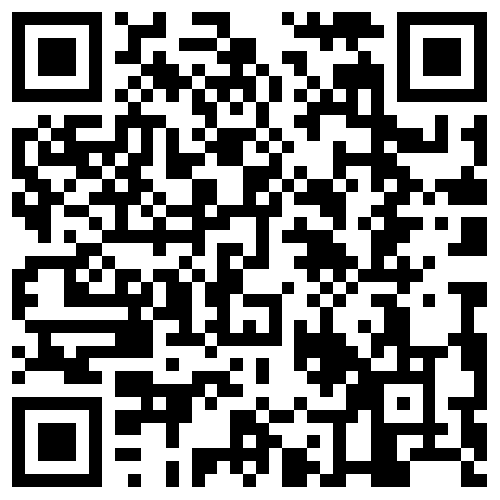
\includegraphics[scale=0.3]{studentionlineqrcode}\\


\subsection{马可波罗计划生}
为中国学生提供的马可波罗计划,旨在欢迎并帮助中国学生入读意大利的大学。得益于本计划,对于想来意大利就读大学的中国学生,即使不懂意大利语也能获得入境签证。该计划要求学生在入读大学课程之前,在参与并遵守该计划的语言学校内学习10-11个月的意大利语课程。\\
您可以在佩鲁贾外国人大学、锡耶纳外国人大学、罗马第三大学、“Dante Alighieri”协会(即但丁语言学校)、雷焦卡拉布里亚外国人大学参加针对马可波罗计划生的意大利语课程。您还可以参加其他参与并遵守马可波罗计划的意大利大学的意大利语课程,部分私立语言学校也可以提供该课程。\\
\textbf{值得注意的是,}从2022/23学年起,马可波罗计划生将不再享有任何专用名额,您需要与居住在其他非欧盟地区的学生平等竞争。\\
计划生注意事项:
\begin{itemize}
\item 抵意后,必须在您预注册文件中指定的时间参加意大利语课程,不得参加非您预注册语言学校的意大利语课程 
\item 马可波罗计划生必须通过上述意大利语课程的考试,以至少达到由欧洲委员会承认的B1水平,并且获得以下意大利语证书之一:CELI B1(佩鲁贾外国人大学)、CILS B1(锡耶纳外国人大学)、PLIDA B1(但丁语言学校)和CERT.IT B1(罗马第三大学)。无论您选择的语言学校的课程进度安排如何,您都必须在2022年12月30日之前通过至少B1水平的语言考试。(注意:如语言学校拥有独立语言证书,则只能提供该校的语言证书。例如您在佩鲁贾外国人大学参加语言课程,则您只能提供CELI B1语言证书。如语言学校没有独立语言证书,您可以提供以上四种中任意一个博洛尼亚大学认可的证书)
\item 您必须通过Studenti Online验证您的语言证书。访问Studenti Online,选择“Bandi”,随后选择“Programma Marco Polo per studenti cinesi a.a. 2022/23 - verifica certificati di lingua italiana”,上传您的语言证书和您的护照的PDF电子版。国际生办公室将对其进行审查,并在Studenti Online上发布结果。审查日期为2022年6月1日至2022年12月30日。如果因必要原因,您无法在此期间提供证书,请联系国际生办公室(internationaldesk@unibo.it)
\item 您需要在入学时,或无论如何都必须在2023年2月28日之前,将证书交付给您所就读专业的秘书处
\item 马可波罗计划生无需、也不得参加博洛尼亚大学为非欧盟学生提供的意大利语测试
\item 您不能提交非上述所列的意大利语水平证明
\item 请记住,马可波罗计划生只能注册以意大利语授课的学习课程。
\end{itemize}
%%%%2022.05.24
\subsection{参加意大利语考试或持有意大利语证书 (免考)}
正式注册大学的另一必要条件是新生的意大利文水平(如果意大利语授课)。未持有大学认可的意大利文证书的新生必须在九月初,专业考试之前,参加一项由各学院举办的意大利文水平测试,通过后方可注册。若持有大学认可的意大利文证书,则只需在前往学院秘书处正式注册时(既通过专业考试后)提供证书的复印件即可。(备注:计划生有B1 证书免考,国际上则需要持有 B2 证书,否则需要加试意大利语测试) 




\subsection{无专业入学考试的情况}
如果新生选报的专业本学年未设置入学考试,新生只需在 Almawelcome 网上正式注册,开放之后办理注册入学(immatricolazione)手续即可。值得注意的是,部分专业可能出现有入学考试,但申请名额未满,考试不必进行的情况,此时新生仍需 按照有入学考试的情况报名申请缴费,然后等待公布考试成绩的日期之后办理正式入学手续。 
\subsection{正式注册入学}
从指定日期起,新生(如有入学考试则需是通过入学考试的新生)可开始办理大学正式注册入学手续。新生先在 Almawelcome 网站上填写并打印入学申请表格,打印第一期学费的缴费单(每学年可选分期支付或一次付清)后到银行缴费,最后到所属秘书处交材料完成所有入学手续并领取学生手册及学生卡。 

所需材料:
\begin{itemize}
\item 填写好并签名的入学申请表格 
\item 缴纳第一期学费的银行收据 
\item 意大利文水平证书(如果未参加大学组织的意大利文水平测试) 
\item 经翻译双认证的高中毕业证书或毕业证和学位证(从大学毕业时取回)
\item 个人寸照
\item 申请居留的回执
\item 护照复印件 
\end{itemize}




\section{入学之后}
大学网站系统发达,各类信息应有尽有。Bologna 大学网站:www.unibo.it 。关于个人信息管理,可以登录, studenti.unibo.it 之后可以, 预约考试(AlmaEsami),交学费,开注册考试证明(Autocertificazione, 当办居留的材料, 申请语言学习(意大利语,英语) 。。。
如果想要快速找到自己专业的网站,推荐通过谷歌搜索,输入“专业名称 unibo”即可。在自己专业的网站上能查到详细的课程表(Orari di lezioni),学习计划(Piano di studio),在学习计划里面能找到细致的课程描述,参考书,考试方式介绍等等。

\subsection{ALMAWIFI 无线网}
ALMAWIFI 是博洛尼亚大学提供的无线网,覆盖所有校区和学生宿舍,注册生都可以登录。登陆无线网需要大学发的用户名及密码,账户格式 ming.xing@studio.unibo.it . 无线网的下载速度非常快,可能1秒好几mb,但是不支持P2P种子下载。连接大学无线网的方法: 选择大学无线网Almawifi,用户名和密码分别为登陆大学账户的邮箱及密码。

\subsection{次年注册手续}
入学一年以后,直至取得新的学位之前,学生都必须无条件的按年缴付学校规定的学费。学费缴付之后,即成功注册了新一学年的学习。除此之外,外国学生还需要注意,旧的居留证过期后,应随时向秘书处递交更新之后的居留证复印件,或者新的居留证申请回执复印件,因为若缺少有效的居留证件,新一年的注册将不会被系统识别,这将会影响到日后考试的注册以及分数登记(verbalizzazione)。 居留条的递交能保持你的学籍3个月有效。

\subsection{学费}
学费单可从 studenti.unibo.it 上,登录之后打印。通过上面的支付码可在意大利境内任何一家 UniCredit 银行缴付学费。同时,也可利用信用卡进行网上学费缴纳。学费须在截止日期前缴付完毕,若逾期未交,将处以几十欧的罚款。 

\subsection{学分制系统介绍}
本科课程学制一般为三年制,总共需要修满180 学分(cfu - crediti formativi universitari),每年60学分的工作量。研究生课程学制一般为两年制,共120学分。研究生入学要求本科课程和研究生的相匹配,如果缺少一些必修学分,往往会收到面试评估,面试过的话才能读研,否则得重新读本科。 

\subsection{选课及学习计划(Piani di studio)}
每一个专业均为学生安排了必修课程和自选课程 (attività formative opzionali) ,学生可以按各自的兴趣,在给定的范畴内选择自己喜欢的课程、实习或研讨活动等(insegnamenti, tirocini, laboratori, seminari, ecc. ) 。选课要求所有的注册生在学校规定日期内,向系秘书处 (Segreteria della facoltà) 递交自己的选课结果,除此之外,大学网站上也开通了有关学习计划的相关网页,学生们可以直接在网上进行填写,具体操作如下: 登陆 https://studenti.unibo.it/ 然后选择 login, 输入自己大学的 username 和 password 之后, 便可以进入 studenti online 页面,选择 piano di studio 即可开始选课。一般在选课截止之前,学习计划的相关网页都会允许学生自由登陆, 并对之前的选择进行修改。一旦选课截止,该网页便会关闭。之后所有关于选课的问题,均须到秘书处咨询解决。每一学年都有选课的机会,但每一学年的注册生,只可选择或修改本年度或往年的学习计划,例如,刚注册的新生只可递交第一学年的学习计划,不能也无权选择第二学年的学习计划,但第二年的注册生,除了可为本年度课程制定学习计划外,还可对第一年已选择的课程进行修改。需要注意的是,学习计划的生效,只针对大学的正式注册生,即已按时缴付学费的学生, 否则,即便递交了学习计划,也会被认为无效。此外,若某年度课程中有待选项目,则学生必须递交过学习计划后,该年度的所有课程对应的考试才会生效,也就是说,若考试通过,可被系统识别,否则系统检测不到这些课程便会显示错误(包括该年度 内所有的必修课,若不递交学习计划,系统也同样不能识别)。学习计划的填写和递交日期,每年都不尽相同,具体详情请查询学院相关网页以便获得准确信息。 

\subsection{考试制度}
考试采用 30 分制,即 30 分为满分,及格分18 分,有时教授为表扬考试出色的学生,除了给他们打 30 分,后面还要加上“Lode”,以示不同。值得注意的是,以自然科学系为例,换成美国的ABC档的话,30L属于A档,29-30属于B档,26-29属于C档,所以你会发现身边意大利人的考试分数接近30的特别多。
考试之前,学生须提前5天在网上预约 (prenotazione) 。考试结束后,预约的界面分数登上了,才算彻底的结束。一般情况下,教授都会为学生统一安排时间进行登分(verbalizzazione)。
所有的专业都会按照学校的要求,在一个学年内,为每门课程安排大约5次考试机会(5 appelli) 。因此,在课程结束之后的一年时间里,若对某次考试成绩不满意,尽可注册下一次的考试,直至考取满意的分数,再请教授把成绩登入系统和记分册。需要注意的是,许多教授在给学生登记成绩时,有特殊的规定:对那些参加过若干次考试的学生,只允许这些学生登记最近一次通过考试的成绩,并不择优登记,也就是说,即使前几次考试的成绩都高于最近的这一次考试成绩,也只能登记最近的这次成绩(当然,前提是成绩在 18 分以上,包括 18 分), 因此,在决定参加下一次考试之前,最好权衡之后再行动。 只有已经注册的学生(即已缴纳学费并在秘书处留下有效居留证复印件)及已将待考科目纳入学习计划的学生,方可参加该门考试,否则,即使考试通过也无法对成绩进行登记。 
有时,教授会特别针对跟班上课和在家自学的同学,准备不同的试卷,因此在注册考试时,需特别留意。对于分阶段上课的同一门课程,最后只登记一个综合成绩。

\subsection{毕业论文/设计}

毕业时间:每学年都有 3 次毕业机会,每个学院毕业时间,毕业机会次数都可能不一样。需要单独查询,以下为大体研究生毕业时间。
\begin{itemize}
\item 第一阶段:7 月 12 日~20 日
\item 第二阶段:10 月 17 日~22 日 11 月 15 日~30 日 12 月 10 日~17 日
\item 第三阶段:3 月 15 日~31 日
提交毕业申请时还需交付毕业证书的定制费 (Pergamena) 
\end{itemize}

\noindent 提交毕业申请的截止日期(对应上述 3 个阶段): 
\begin{itemize}
\item 第一阶段:5 月 15 日
\item 第二阶段:9 月 15 日
\item 第三阶段:1 月 15 日 
\end{itemize}
迟到提交会收到罚金。

\subsection{实习 (Tirocinio)}
学校会不定期在网站上张贴布告(Bando) ,向学生提供各种有关实习机会的消息,学生可根据自身兴趣选择参加,一般需递交个人简历,或进行面试。 实习与毕业论文,在与相关导师协调后,也常能结合在一起完成。实习的选择范围很宽泛。除了学校推荐的公司和企业外,学生还可自行寻找实习对象,但该实习对象须与校方签订相应合同 (Convenzione),实习方可生效。此外,在校生与毕业后不满 18 个月的毕业生均可参加这些实习项目。对于在校生,实习往往是必须的,因此学校方 面对实习的时间也有相应规定,每工作 25 小时即可 
赚取一学分,例如,若要获得 10 学分,则一共需要工作至少250 小时。而对于毕业生,学校方面则没有任何时间限制。 
\subsection{留学回国人员证明}
在毕业后如何到罗马的中国驻意大利大使馆教育处开具此证明 
前提准备: 需要去当地学联网站(Bologna 大学中国学联的网站是:www.boxue.it)或学联办公室领取并填写《赴意大利留学人员登记表》。

\section{学费减免及奖学金}

大区学习权利机构 ER-GO 为学生提供各项便利, 包括学费减免、奖学金、住宿、食堂及国际交换协助等。ER-GO 每年七月公布各项目的公告及申请截止日期, 请关注网站 www.er-go.it 。 
学费减免分多等,最多减免一半,只有在有奖学金的情况下,学费才全免。头一年申请凭借家庭状况排名,从第二年往后,根据学分排名,同样学分时,根据平均分排名。奖学金按租房情况分 In sede 、Pendolare 和 Fuori sede 三大类,金额递增。In sede,为黑户,pendolare,房东开免费居住证明,fuori sede,有正规房租合同的付费证明。In sede收到的奖学金是Fuori sede的一半。所以一定注意在截止日期之前提交合同复印件。对于房产在中国,父母工作在中国的大部分留学生来说,都是 fuori sede 的选项。

\subsection{申请基本流程}
\begin{itemize}
 \item 网上填写申请表格 \\https://www.er-go.it
 \item 点击 login, 输入大学 username 和 password
 \item 进入主页面, 点击选项: "per compilare/visualizzare il modulo per I benefici a concorso a.a.
2016/2017"
 \item 在截止日期前确认表格中所填写内容并提交。
 \item 打印申请表格签字 
 \item 将申请表附上各项证明材料在截止日期前寄出 
 \item 等候 ER-GO 公布结果:往往11月初左右,如果材料有问题,可以补充。12月底开始发第一批奖学金。
 \item 8月10号之前达到要求学分,会收到第二批奖学金。
\end{itemize}
注:如果是需要申请学生宿舍的同学,请
务必将所有认证材料在 8 月 10 日之前办好并寄给 ER.GO, ER.GO 需要提前审核材料并且 在两个星期之后公布第一批入住宿舍资格名单,如果又缺少材料或者材料有问题的同 学,ER.GO 将会给你发补全材料的信件,如果在规定日期到期之前将材料补全并且通过 审核,则可以在第二批名单(最终名单)中获得入住宿舍的资格。

\subsection{申请奖学金的基本学分要求}

\subsubsection{学分要求}

\subsubsection{本科}
\begin{tabularx}{\textwidth}{ |X|X| }
  \hline
  年份 & 要求学分\\
  \hline 
  第一年  & 25  \\
  第二年  & 80  \\
  第三年  & 135  \\
  \hline
\end{tabularx}



\subsubsection{研究生}
\begin{tabularx}{\textwidth}{ |X|X| }
  \hline
  年份 & 要求学分\\
  \hline 
  第一年  & 30  \\
  第二年  & 80  \\
  \hline
\end{tabularx}


\subsubsection{借学分(Bonus)}
因为特殊情况,没有达到指定要求学分的同学也可通过借学分的方式获得奖学金。可借学分如下表。一共只能借一次,借剩下的学分可以来年接着用。\\
\begin{tabularx}{\textwidth}{ |X|X| }
  \hline
  年份 & 可借学分\\
  \hline 
  第一年  & 5  \\
  第二年  & 12  \\
  第二年  & 15  \\
  \hline
\end{tabularx}

\subsection{家庭经济状况证明需准备之材料}
\begin{itemize}
 \item 家庭成员亲属关系证明(成员、关系、人口,父母离异亦须证明)
 \item 各家庭成员上一年的年度收入(无业务收入等都须开出相应证明) 
 \item 家庭拥有的房产证明(如无房产则提供租房合同,分期付款未清证明等)
\end{itemize} 

\subsection{办理奖学金的注意事项}
以上各项材料均需公证翻译成意大利文并经双认证。过去 Er.Go 开始办理奖学金的时间是从7月中旬开始,每年略有变动,详情请关注 ERGO.it 或者Bologna大学中国学联官方论坛公告(www.boxue.it/bbs ) 


\section{大学的福利}
入读博洛尼亚大学后,你将不仅可以享受到一流的教育,同样可以享受大学提供的福利,以便你体验这边的生活、优惠并探访名胜古迹。

\subsection{影院、博物馆和剧院等}

博洛尼亚的大部分影院、博物馆和剧院均有学生票,购买时会要求你出示大学徽章(badge),也有可能要求你提供本学年的入学证明,在访问前请仔细查看其官网的要求。入学证明可以在Studenti online网站登录下载。

\subsubsection{大学博物馆系统 - SMA}
博洛尼亚大学拥有非常发达的博物馆系统,几乎每个学院都有自己的博物馆。包括解剖学博物馆、矿物学博物馆、物理学博物馆以及大学植物园都是非常值得一看的。大部分博物馆对于本校学生均为免费开放。具体信息及预约访问的方式可以查看各博物馆的页面。\\
官网地址:https://sma.unibo.it/it

\subsubsection{爱乐学院音乐会}
博洛尼亚爱乐音乐学院Accademia Filarmonica di Bologna为博洛尼亚大学的学生提供了特殊的优惠,可以在音乐会前半小时在Via Guerrazzi,13的售票处以5欧元的价格购买门票。座位有限。\\
该优惠仅针对部分音乐会有效,详情请访问爱乐学院官网。\\
官网地址:https://accademiafilarmonica.it/

\subsection{交通福利}

\subsubsection{Almabike}
Almabike是一款男女通用的城市自行车,专为满足大学生的需求而设计。该项目由环境部资助,为研究大都市区域的空气质量,经过博洛尼亚大学学生的初步招标,一位专门从事该主题的知名设计师开发了这样一款个性化的自行车。AlmaBike是在特定招标后生产的,其配备了GPS防盗传感器。\\
Almabike可用于科学研究,其配备能够检测空气质量、噪音和环境参数的传感器。其隶属于DICAM-Strade研究部门、AUTC以及Technion-Israel Institute of Technology合作开展的一项研究项目的一部分。\\
该项目的目标是:
\begin{itemize}
 \item 试验用于测量与博洛尼亚市道路系统相关的环境质量数据的准时和动态系统;
 \item 测量空气质量意识在选择工作方针或服务转移所采用的路线方面的相关性; 
 \item 对骑自行车者的路线选择进行基础设施和道德选择类型的多因素分析。
\end{itemize} 

委托使用Almabike的学生必须:
\begin{itemize}
 \item 停车期间将其固定在自行车架上,确保自行车安全;
 \item 保证自行车整体质量和部件效率的维护,自费提供普通和特殊维护; 
 \item 确保GPS跟踪器的正确操作,提供相应的充电,充电周期约为48小时。
\end{itemize}
如果你想参与申请Almabike,或者想了解更多信息,请扫描下方二维码,并参阅该页面。\\
\\
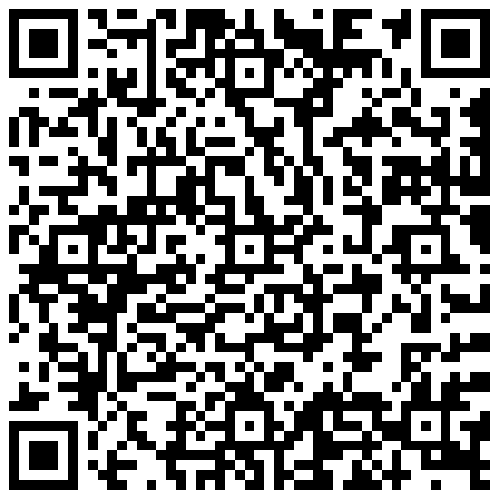
\includegraphics[scale=0.3]{almabikeqrcode}\\
%%https://site.unibo.it/multicampus-sostenibile/it/mobilita/almabike

\subsubsection{Tper公交年票}
博洛尼亚大学学生在已注册的学年,可以以180欧元的价格购买到Zone3(包括奥扎诺市)的城市公共交通年票,该优惠也对博士生开放。选择博洛尼亚作为交换地点的交换生将能够在交换期间以象征性的10欧元购买一张交通票。要购买该年票,您需要使用您的账户登录Studenti Online,选择Richiesta abbonamento autobus,随后跟随流程填写信息并预约前往Tper服务点领取。如果您拥有卡片,请在购买时填写卡号,在首次使用前也请前往Tper服务点激活。\\
\\
大学也提供了更高的99欧年票折扣,但是是有名额限制的。其申请方法请扫描下方二维码,并参阅我们的官网页面。\\
\\
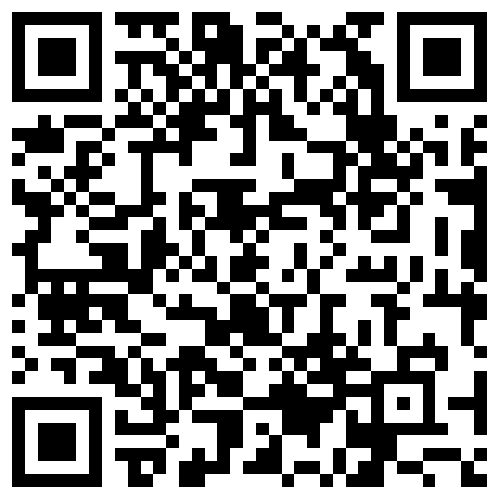
\includegraphics[scale=0.3]{tper99qrcode}\\
%%https://asscubo.it/2021/11/07/tper99/

\subsection{大学语言中心 - CLA}
大学语言中心对就读博洛尼亚大学的国际学生和交换生有条件提供免费的意大利语课程。一般为首轮课程免费,且不包括就读高等教育课程和研究项目的学生。有关的信息和申请方式、时间表等,请扫描下方二维码并参阅此页面。\\
\\
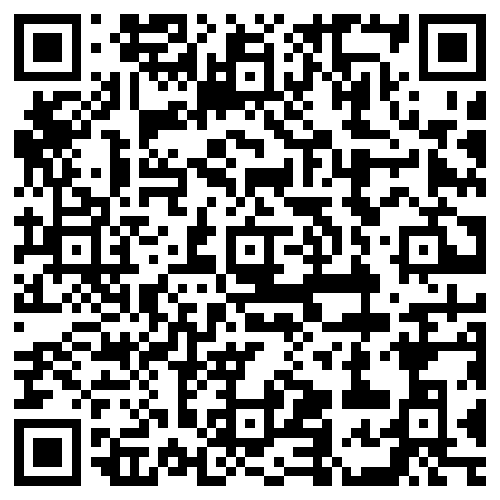
\includegraphics[scale=0.3]{corsiclaqrcode}\\
\\
同样,大学语言中心也提供了其它语言的相关课程,报名方式等更多信息均可前往其官网查看。\\
官网地址:https://centri.unibo.it/cla/it\\

\subsection{YoungERcard}
YoungERcard卡由艾米利亚-罗马涅大区政府提供,针对14-29岁之间的年轻人。使用该卡可以在约2000个合作机构及商店获取折扣和优惠。申请该卡为免费,且流程简单。有关信息请参阅其官网。\\
官网地址:https://www.youngercard.it/

\subsection{大学音乐学院}
大学音乐学院、合唱团和管弦乐团,Il Collegium Musicum, Coro e Orchestra dell’Università di Bologna,为大学生提供了在年轻、充满活力和国际化的环境中分享他们对音乐的热情和好奇心的机会。音乐是一种通用语言,可以让不同现实之间相遇和交流,是文化深化和丰富阅历的机会,可以丰富你的大学体验。\\
如果想要加入合唱团或管弦乐团,或是前往欣赏音乐会,请参阅其官网。\\
官网地址:https://collegiummusicumbologna.com/

\subsection{Wi-Fi}
\subsubsection{ALMAWIFI}
ALMAWIFI是博洛尼亚大学无线网络的名称,它允许大学社区使用WiFi系统,直接从移动设备访问互联网和大学的在线服务。\\
所有博洛尼亚大学的教授、学生、技术管理人员、研究员、博士生和认可的合作者均可使用DSA凭据(等同于登录Studenti online的账户)来访问ALMAWIFI。\\
具体信息、使用方法等,请扫面下方二维码,并参阅该页面,在页面的右方附件中,有各系统访问ALMAWIFI的详细指南。\\
\\

\includegraphics[scale=0.3]{almawifiqrcode}
%%https://www.unibo.it/it/servizi-e-opportunita/studio-e-non-solo/wi-fi/almawifi
\subsubsection{Iperbole}
Iperbole Wireless由博洛尼亚市政府提供。在博洛尼亚的部分室外及室内地区均已覆盖该网络,如果您想要使用,只需连接到名为iperbole的无线网络即可,无需身份验证。\\
在对提供服务的技术设备进行预防性、普通和特殊维护所必需的暂停期间,将不保证服务。\\
有关其提供服务的区域,请访问官网。\\
官网地址:https://www.comune.bologna.it/notizie/wireless

\subsubsection{Eduroam}
Eduroam - 教育漫游,是一项为国际科学界用户提供安全无线网络访问的服务。它是一个带有“eduroam”标识(SSID)的无线网络,受 WPA2/AES 协议和PEAP身份验证保护。Eduroam成员机构(如博洛尼亚大学)的用户访问另一家成员机构时,可以通过其凭据(用户名和密码)使用其本地无线网络,而无需在主办机构进一步办理手续。\\
该服务提供给博洛尼亚大学的教学和研究人员、研究员、博士生、技术管理人员和前往该服务所涵盖机构的学生,以及属于Eduroam机构的博洛尼亚大学的客人。\\
有关其具体信息和使用方法,请扫描下方二维码并参阅该页面。\\
\\
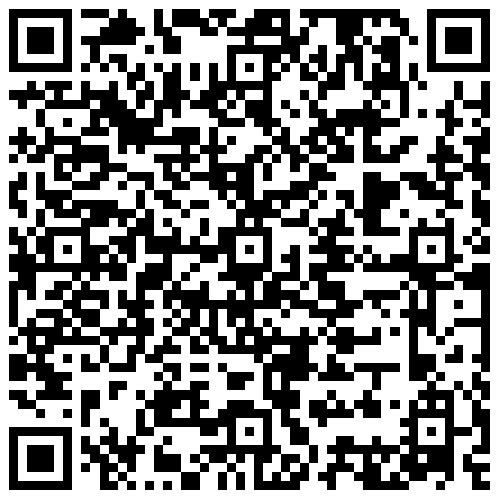
\includegraphics[scale=0.3]{eduroamqrcode}
%%https://www.unibo.it/it/servizi-e-opportunita/studio-e-non-solo/wi-fi/eduroam-education-roaming

\subsection{大学周边}
大学周边商店,即UniboStore,销售各式各样含有大学元素的商品。其出售的Alma Mater Studiorum服装和配饰系列是与从事体育运动的国内和国际领先公司Macron合作创建。
如果想要购买,可以选择网上浏览或者前往线下商店。\\
官网地址:https://www.unibostore.it/\\
商店地址:Piazza Verdi, 2/A - 40126 - Bologna\\
营业时间:周一至周五 9:00-19:00

\subsection{图书馆系统}
\subsubsection{SBA}
大学图书馆系统 - SBA,是负责协调图书馆、图书收藏以及书目和文献服务的大学机构,博洛尼亚大学几乎每个学院都有图书馆。如果你想要借阅图书,可以通过图书馆官网首页的检索系统查找是否有这本书、在哪个图书馆、并且可以在线预约领取时间。大学同样拥有数量即为可观的电子版资源和文献。\\
官方网站:https://sba.unibo.it/it\\
\subsubsection{SBN/UBO}
同时大学还和大区及市立图书馆合作,成立了SBA/UBO系统方便博洛尼亚大学的学生使用,其官网主页同样拥有检索系统。\\
官方网站:https://sol.unibo.it/SebinaOpac/.do

\subsubsection{AlmaRE}
AlmaRE拥有意大利境内最大的数据库、电子期刊和电子书集合,也涵盖了利基学科领域。其拥有:\\
超过5万种电子期刊;超过370个书目、全文、事实和引文的数据库;超过64万本电子书,包括手册、百科全书、词典、参考书等。\\
同时大学还和包括剑桥大学出版社、美国化学学会、《自然》杂志,中国知网等几十家权威学术机构合作并订购了资源。\\
要查看更多信息,请访问AlmaRE官网:\\
https://sba.unibo.it/it/almare\\
要查阅资源,请访问其检索系统:\\
https://almastart.unibo.it/primo-explore/search?vid=39UBO\_VU\\
\textbf{注意!}有关中国知网的资源,请检索“CNKI”。

\subsection{软件折扣}
\subsubsection{Prezi}
Prezi是一个允许您以简单直观的方式创建演示文稿的系统。每个带有.pez扩展名的演示文稿都可以从具有Internet连接的任何计算机投影,或者,如果脱机或保存在USB设备上,则可以通过程序为Windows和Mac环境自动生成的播放器投影。\\
对于博洛尼亚大学的学生,通过机构电子邮件name.surname@studio.unibo.it注册,可以免费获得EDU Enjoy版本,并以折扣价获得EDU Pro版本。\\
注册网址:https://prezi.com/pricing/edu/

\subsubsection{MATLAB}
MATLAB - 校园许可证:根据与MathWorks的协议,大学已激活MATLAB Campus许可证,所有教师、研究人员、技术管理人员和学生都可以在他们的计算机上安装MATLAB和Simulink应用程序,并参加免费的在线培训课程。\\
MATLAB是一个用于数值计算、统计分析和仿真的开发环境,全球有数百万人使用,其主要用于经济学、工程、数学、物理、医学、生物学等领域。Simulink是用于多域仿真和基于模型的设计的图形环境,与MATLAB集成。\\
该软许可证可供博洛尼亚大学社区的所有成员使用,包括:教授、研究人员、技术管理人员和学生,简而言之拥有大学凭证(@unibo.it 或@studio.unibo.it)的成员。\\
该许可证包括MATLAB和Simulink应用程序以及工具箱。完整列表可在其官网的博洛尼亚大学页面上找到。该许可证包括来自 MathWorks 的技术支持(使用电子邮件地址support@mathworks.it)。也包括了提供免费的在线培训课程。\\
\textbf{注意!}仅允许用于教育或公共研究活动(结果必须是公开的,而不是公司专有的)。因此它不能用于商业活动。安装软件的机器必须归博洛尼亚大学或个人所有。不允许安装在其他机构或研究中心的计算机上,即使大学与他们有持续的合作。\\
注册网址:https://it.mathworks.com/academia/tah-portal/alma-mater-studiorum-universita-di-bologna-1122528.html

\subsubsection{Microsoft Office 365}
根据与微软的协议,博洛尼亚大学的所有学生都可以免费使用Office365套件。\\
Office 365是一套个人生产力工具,包括电子邮件管理、专业编辑、电子表格和演示文稿管理、文档共享等。\\
Office 365可供所有在博洛尼亚大学定期注册的学生使用,并可通过他们的大学凭证 (@studio.unibo.it) 在portal.office365.com上访问。当学生与大学的关系终止后,将保留仅使用电子邮件的可能性。\\
随着研究的结束,通过博洛尼亚大学与Microsoft的协议安装在个人计算机上的Office产品许可证的有效性也将终止。要继续使用产品,您必须根据微软的商业条件购买许可证。\\
大学提供的许可证包括:
\begin{itemize}
 \item 能够使用Office 的在线版本,其中包括例如Word、Excel、PowerPoint、Outlook(邮件、联系人、日历、任务);
 \item 能够下载和安装最新版本的Office; 
 \item 访问Onedrive:用于在所有设备上编辑和共享的文档、照片和视频的云存储空间;
 \item Skype for Business:即时通讯软件、音频和视频通话、在线会议和演示、可用性信息和共享,供您在组织内使用。
\end{itemize}
要下载并使用Office365套件,请访问微软官网,并使用你的大学凭证(即登录Studenti online的账户)登录。\\
微软官网:https://www.microsoft.com/

\subsubsection{其他}
很多软件对学生都有折扣和优惠,例如ADOBE旗下的软件、Cinema 4D、AutoCAD等,有关信息请访问各软件官方网站查看。

\subsection{如果您是一位母亲}
博洛尼亚大学拥有向母亲开放的母乳喂养区,对女学生、教师、技术管理人员、博士生、研究员和任何需要安静空间来母乳喂养的新妈妈们、以及她们的探亲家庭成员(例如在毕业典礼期间)开放。\\
空间内有:更衣台、水槽、奶瓶加热器、一个供年长兄弟姐妹使用的小型游乐区和一个供陪伴他们的人使用的等候区。\\
地址和时间:\\
Via B. Andretta, 4 (ex-Belmeloro 10-12) Bologna\\
开放时间:周一至周五 9:00 至 19:00\\
Via Zamboni 33 Bologna, 即il Museo di Palazzo Poggi\\
开放时间:周二至周五 10:00 至 16:00 - 周六和周日 10:00 至 18:00\\
Via Zamboni, 63 Bologna, 即la Collezione di Geologia “Museo Giovanni Capellini”\\
开放时间:周二至周五 10:00 至 16:00 - 周六和周日 10:00 至 18:00\\








